
%------------------------------------------------

\newpage

\section{Gaussian random number generator}
\label{exer:gaussian_random_number_generator}

\subsection{Central limit for Gaussian random number generator}

\begin{enumerate}
	\item Generate $10^{8}$ sets of $n$ uniformly distributed random variables in $[0, 1)$, with $n = \{ 1, 2, \cdots,10 \}$.
	\item For every $n$, populate a histogram with the $10^{8}$ sums of the $n$ generated random numbers.
	\item Plot the histogram in linear and log-scale. 
		\marginnote{Do you notice anything?
		
		One can demonstrate that the distribution will be cut off at $\pm \sqrt{3n}$.}
\end{enumerate}

(Figure~\ref{fig:gaussian_random_number_generator} and~\ref{fig:gaussian_random_number_generator_logy})

\begin{figure}
	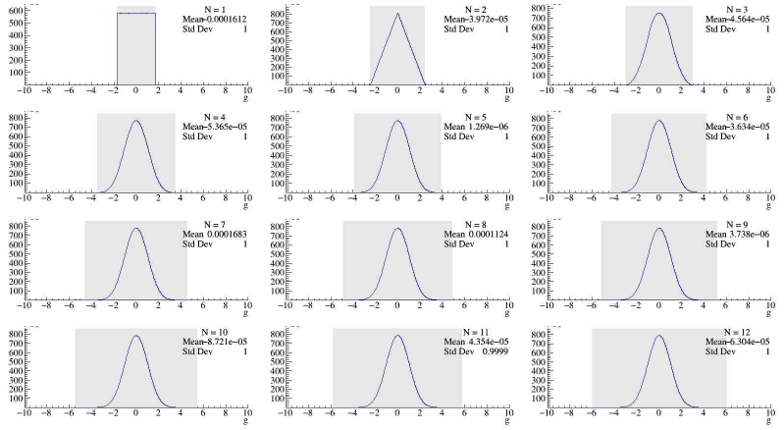
\includegraphics{exercise/gaussian_random_number_generator.png}
	\caption[Central limit for Gaussian random number generator.][6pt]{Central limit for Gaussian random number generator.}
	\label{fig:gaussian_random_number_generator}
\end{figure}

\begin{figure}
	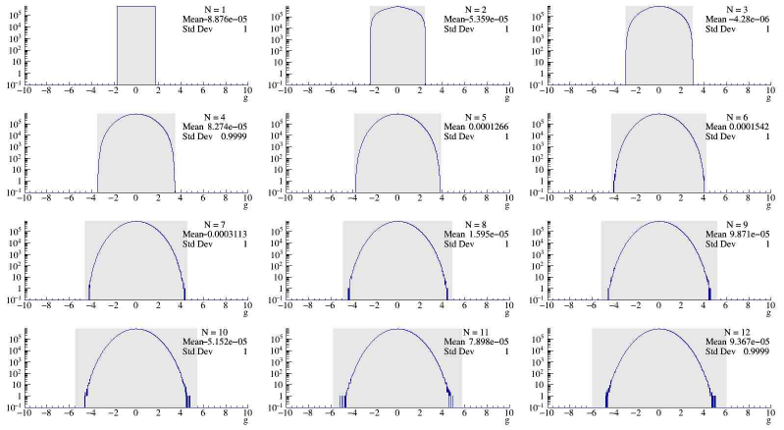
\includegraphics{exercise/gaussian_random_number_generator_logy.png}
	\caption[Central limit for Gaussian random number generator with log-scale.][6pt]{Central limit for Gaussian random number generator with log-scale.}
	\label{fig:gaussian_random_number_generator_logy}
\end{figure}

($\hookleftarrow$ \ref{subsec:central_limit_theorem})
